
\documentclass[times, 10pt,twocolumn]{article}
\usepackage{main}
\usepackage{times}
\usepackage{amsmath}
\usepackage{amssymb}
\usepackage{booktabs}
\usepackage{graphicx}
\graphicspath{{figures/}}

\pagestyle{empty}

\begin{document}

\title{Increasing Reward Quality and Density for Verifiable Rewards\\
       via Master/Novice Divergence}

\author{Ana Carolina Ramos Cunha\\
Technical University of Munich\\
\and
Leonard Evers\\
Technical University of Munich\\
\and
Leonhard Driesch\\
Technical University of Munich\\
}

\maketitle
\thispagestyle{empty}

\begin{abstract}
Reinforcement learning for large language models on verifiable tasks---mathematics,
code, and other domains with binary correctness checks---suffers from reward
sparsity: only the final outcome receives a signal, leaving credit assignment
across long chains of thought unresolved. We investigate a Master/Novice
framework that compares a strong policy to a structurally matched but
capacity-reduced \emph{Novice}, obtained by tensor disentanglement of the
Master's MLP weights, and asks whether their per-token divergence identifies
the steps that deserve credit. We contribute (i)~the conceptual framework and
its central, testable hypothesis; (ii)~an end-to-end \texttt{NoviceModel}
pipeline that scales tensor disentanglement to Qwen3.5-4B and bakes Novices at
any rank fraction from a single checkpoint; and (iii)~a hypothesis-first
causal evaluation on MATH-500. Three intervention designs of
increasing strength---handing generation over to the Novice, perturbing single
tokens, and corrupting whole reasoning steps---consistently fail to reject the
null: disagreement positions carry no more outcome leverage than depth-matched
control positions (McNemar $p{=}1.00$; Fisher $p{=}0.80$), and the Novice's
specific token choices are no more damaging than generic perturbations
($p{=}1.00$). The only reliable effect is local: disagreement positions are
more fragile in the immediate continuation, and this effect survives
controlling for Master entropy ($t{=}2.35$). We report these negative results
precisely, characterize a coherence cliff that constrains usable Novice ranks,
and discuss what they imply for divergence-based reward densification.
\end{abstract}


\Section{Introduction}

Large language models (LLMs) trained with reinforcement learning often receive
only a sparse, verifiable reward at trajectory end---correct or
incorrect---while intermediate tokens receive no direct feedback. This
\emph{reward sparsity} impedes sample efficiency and credit assignment: the
policy cannot tell which reasoning steps were load-bearing and which were
routine~\cite{cui2025prime}.

Recent work densifies rewards without human step labels by exploiting structure
already present in the task or the model: partial test-case success in
code~\cite{wang2026verpo}, implicit process rewards trained from outcome labels
alone~\cite{cui2025prime}, teacher--student divergence in
distillation~\cite{xu2026tip}, and the observation that a minority of
high-entropy ``forking'' tokens concentrates most of the learning signal in
RLVR~\cite{wang2025forking}.

This paper explores a complementary idea: construct a weaker \emph{Novice} from
the same base weights as the \emph{Master} via tensor disentanglement, compare
their next-token distributions on successful Master rollouts, and upweight
positions where the two diverge---on the premise that such steps rely on
knowledge the Novice lacks and therefore deserve higher credit. Unlike an
externally trained reward model, the Novice shares architecture and tokenizer
with the Master and offers a continuous knob (the retained rank fraction) for
how weak the comparator should be.

Our contributions are of three kinds. \emph{Conceptually}, we formalize the
Master/Novice framework and reduce its promise to a single testable hypothesis:
divergence positions have higher causal leverage on the final outcome than
matched non-divergence positions. \emph{Methodologically}, we implement an
end-to-end \texttt{NoviceModel} pipeline---disentangle, save/load, bake to a
chosen rank, and generate---validated from MLP-scale prototypes through
Qwen3.5-4B, together with a ladder of three causal intervention designs for
testing per-token credit signals before committing to RL training.
\emph{Empirically}, we characterize the disentanglement and Novice-quality
landscape (learning-rate sweep, MMLU rank sweep, a generation-level coherence
cliff) and report a consistent, statistically quantified negative result on the
central hypothesis, alongside one genuine positive: a local fragility effect at
disagreement positions that is not explained by Master entropy alone.


\Section{Related Work}

We group prior work by where the dense signal comes from: the \emph{task}
(verifiable structure) or the \emph{model} (internal statistics). For each line
of work we focus on its relation to our approach; we refer to the original
papers for full results.

\SubSection{Dense rewards from verifiable task structure}

\textbf{VeRPO}~\cite{wang2026verpo} densifies code-RL rewards using partial
test-case success. Its central observation is cautionary: the naive dense
signal---the raw test-suite pass rate---can \emph{underperform} sparse outcome
rewards, because redundant easy tests dominate the reward by sheer count (a
\emph{cardinality bias}). VeRPO corrects this with a dynamically calibrated
per-test weighting and re-anchors the result to the end-to-end outcome,
outperforming outcome-only GRPO and RM-based baselines without a learned
reward model. We selected it both as the clearest instance of extracting
density from the \emph{verifier} side and for its lesson that denser is not
automatically better---the same lesson that motivates our causal validation of
the divergence signal before any training. It differs from our approach in
scope and granularity: the signal exists only where partial success is
measurable (currently code) and is assigned per turn, whereas a Master/Novice
comparator is task-agnostic and per token.

\textbf{PRIME}~\cite{cui2025prime} obtains per-token process rewards without
step labels by training an outcome reward model whose log-ratio to a reference
policy is reinterpreted as an implicit process reward, updated online alongside
the policy. It substantially improves sample efficiency over outcome-only RL on
math and code. PRIME is the closest point of comparison for our goal
(token-level credit from outcome supervision only); the difference is that
PRIME \emph{learns} its dense signal, whereas we test whether a fixed,
training-free capacity-reduced copy of the policy can supply one.

\SubSection{Token-importance signals inside the model}

\textbf{High-entropy minority tokens.} Wang et
al.~\cite{wang2025forking} show that in RLVR most chain-of-thought tokens are
low-entropy ``followers,'' while a minority of high-entropy forking tokens
carries the learning signal: restricting policy gradients to the top 20\%
highest-entropy tokens matches or exceeds full-gradient training. We selected
this work because Master entropy is the natural single-model baseline that any
two-model divergence signal must beat; our experiments therefore control for
entropy explicitly.

\textbf{TIP}~\cite{xu2026tip} studies on-policy distillation and identifies
informative tokens along two axes, student entropy and teacher--student
divergence: entropy-only selection is structurally blind to positions where
the student is confidently wrong, and training on under 10\% of tokens---the
low-entropy, high-divergence region alone---nearly matches full-token
distillation. TIP is the closest conceptual
relative of our hypothesis---divergence between a strong and a weak model marks
important tokens---but it operates in distillation, where the teacher's
distribution is the training target itself. Whether the same signal identifies
\emph{outcome-critical} steps for RL credit assignment is exactly the question
our experiments address; our negative results suggest the transfer is not
automatic.

Compared with all four, the Master/Novice comparator requires no additional
training, no task-specific verifier beyond the outcome check, and applies to
any domain with verifiable answers; the price, as our results show, is that the
signal it produces must be validated causally rather than assumed.


\Section{Master/Novice Framework}

\SubSection{Setup and hypothesis}\label{sec:hypothesis}

We treat autoregressive generation as a Markov decision process: state $s_t$ is
the prompt plus generated prefix $y_{<t}$, action $a_t$ is the next token, and
the reward is binary verifiable correctness at episode end. The
\textbf{Master} is the full-capacity policy $\pi_M$. The \textbf{Novice} is
$\pi_N$, derived from the same checkpoint by truncating disentangled MLP
factors to a rank fraction $\rho \in (0,1]$. On a Master rollout
$\tau = (y_1,\ldots,y_T)$ that reaches a correct answer, per-token divergence
is
\begin{equation}
\delta_t = D\bigl(\pi_M(\cdot \mid y_{<t}),\, \pi_N(\cdot \mid y_{<t})\bigr),
\end{equation}
where $D$ may be instantiated as a distributional distance (KL, Jensen--Shannon)
or, in the discrete limit used throughout our experiments, as the
\emph{top-1 flip} indicator
\begin{equation}
\mathrm{flip}_t = \mathbb{1}\bigl[\arg\max \pi_N(\cdot \mid y_{<t}) \neq y_t\bigr],
\end{equation}
i.e., whether the Novice would have emitted a different token at position $t$.
The top-1 flip is one instantiation of the framework, chosen for the
experiments because it is parameter-free and directly interpretable; the
framework itself is agnostic to the divergence measure. This setup---the full
policy generates while its truncated counterpart re-scores the same
states---instantiates the \emph{Observer pattern} of the weight-matrix
disentanglement (WMD) introspection framework~\cite{till2026introspection},
and the top-1 flip corresponds to its discrete \emph{behavioral disagreement}
indicator.

The intended use of $\delta_t$ is as a shaping signal that concentrates credit
on high-divergence steps of verified-correct rollouts. Before such a signal
enters any RL objective, however, its premise must hold. We therefore state it
as an explicit hypothesis:

\medskip
\noindent\textbf{H1 (outcome leverage).} \emph{Positions where the Novice
diverges from the Master have a larger causal effect on final-answer
correctness than depth-matched positions where the two agree.}
\medskip

\noindent All credit-assignment experiments in this paper are direct causal
tests of H1 at increasing intervention strength. We deliberately do not
evaluate any RL training run: if H1 fails, divergence-weighted advantages
cannot concentrate gradient where the outcome is decided, and the training
experiment would be uninformative.

\SubSection{Constructing the Novice via weight matrix disentanglement}\label{sec:wmd}

The Novice must be \emph{policy-preserving}: it should retain as much of the
Master's behavior as a given rank budget permits, so that its remaining
disagreements are attributable to missing capacity rather than to a lossy
construction. The classical route---truncated SVD of each weight matrix,
optimal in Frobenius norm by Eckart--Young---treats the matrix as a flat 2D
array and ignores the multi-dimensional structure of neural weights. We
instead use \emph{Weight Matrix Disentanglement}
(WMD)~\cite{till2026introspection}, following the Master/Novice framework of
Till (sebis/TUM), which adapts tensor disentanglement from numerical linear
algebra~\cite{wei2025tensor} to neural network layers.

Let $X \in \mathbb{R}^{lr \times bc}$ be a decoder-MLP weight matrix whose row
and column dimensions are split into near-balanced factor pairs $(l, r)$ and
$(b, c)$. Writing $M$ for the reshape of $X$ into the 4th-order tensor
$\mathcal{X} \in \mathbb{R}^{l \times r \times b \times c}$ and $P$ for the
index permutation $(l,r,b,c) \to (l,c,r,b)$, WMD re-bipartitions the tensor
with the operator
\begin{equation}
A \equiv M^{-1} \circ P \circ M \colon\;
\mathbb{R}^{lr \times bc} \to \mathbb{R}^{lc \times rb},
\end{equation}
exposing cross-dimensional correlations that the flat matricization hides. A
learnable orthogonal \emph{gauge} $Q \in O(lr)$ is applied to the row space
before re-bipartitioning, and is optimized to concentrate the spectrum of
$A(QX)$ in its leading singular directions. For a target rank $k$, the
optimal disentangler minimizes the energy of the discarded singular tail:
\begin{equation}
Q^{*}_{k} \;=\; \operatorname*{arg\,min}_{Q \in O(lr)}
\sum_{i > k} \sigma_i^2\bigl(A(QX)\bigr).
\label{eq:gauge}
\end{equation}
Because $A$ is an isometry and $Q$ is orthogonal, the total singular energy of
$A(QX)$ is invariant, so \eqref{eq:gauge} directly minimizes the Frobenius
reconstruction error of the truncated layer; the identity gauge $Q{=}I$
recovers plain SVD truncation, so the optimized gauge is never worse. The
rank-$k$ Novice weight is reconstructed by inverting the pipeline,
\begin{equation}
\widetilde{X}^{(k)} \;=\; Q^{*\top}
A^{-1}\bigl(\operatorname{trunc}_k(A(Q^{*}X))\bigr),
\label{eq:bake}
\end{equation}
and the per-layer rank is set by a single global rank fraction:
$k(\rho) = \max(1, \lceil \rho\, m \rceil)$ with $m = \min(lc, rb)$.

The optimization problem \eqref{eq:gauge} admits a closed-form gradient that
reuses one SVD of $A(QX)$ per step~\cite{wei2025tensor}, and can be solved by
Riemannian first- and second-order methods or by alternating minimization
between $Q$ and the low-rank factors. Our implementation (vendored from the
reference disentanglement code) defaults to Adam on a Cayley-parameterized
orthogonal matrix, which maintains exact orthogonality with an inexpensive
backward pass; layers are independent, so all MLP projections are processed in
parallel and their factors streamed to disk.

WMD also supplies the theoretical link between Novice construction and the
divergence signal of Section~\ref{sec:hypothesis}: for a policy and its rank-$k$ truncated
counterpart, the per-state KL divergence is bounded by the discarded singular
tail, $D_{\mathrm{KL}}\bigl(\pi_M(\cdot \mid s)\,\|\,\pi_N(\cdot \mid s)\bigr)
\le \tfrac{L}{2} \sum_{i>k} \sigma_i^2\bigl(A(Q^{*}X)\bigr)$ with $L$ a
network-wide Fisher-information Lipschitz constant, and, at the rank the gauge
was optimized for, the optimized gauge yields the tightest such
bound~\cite{till2026introspection}. Two properties of our pipeline determine
how this applies to the Novices used below. First, baking truncates the
\emph{stored factors} of $A(Q^{*}X)$ before inverting the reshape, exactly the
construction in \eqref{eq:bake}, so the bound itself holds at every bake rank
$\rho$, with the tail read directly off the stored spectrum. Second, because
\eqref{eq:gauge} depends on $k$, the \emph{tightness} guarantee is
rank-specific: a Novice baked at a different $\rho$ than the gauge was
optimized for inherits a valid but not provably minimal bound. We verify
empirically that the gauge's advantage transfers across ranks in our
checkpoint (Section~\ref{sec:characterization}). WMD rather than plain SVD
thus keeps the observed Master/Novice divergence dominated by genuinely
missing capacity rather than by avoidable truncation error.

\SubSection{The \texttt{NoviceModel} pipeline}

The \texttt{NoviceModel} wrapper owns the full lifecycle: load a base causal
LM, swap MLP linears, run disentanglement, persist factors to disk (monolithic
or per-layer sharded checkpoints with a manifest), bake to any $\rho$ via
\eqref{eq:bake}, and delegate \texttt{generate()} to the underlying
\texttt{PreTrainedModel}, preserving KV-cache compatibility. Concretely, for
Qwen3.5-4B's \texttt{down\_proj} ($X \in \mathbb{R}^{2560 \times 9216}$) the
factorization is $(l,r,b,c) = (40,64,96,96)$, so $Q \in O(2560)$,
$A(QX) \in \mathbb{R}^{3840 \times 6144}$, and $m = 3840$; baking at
$\rho{=}0.25$ keeps $k{=}960$ singular directions. The stored per-layer
factors $(Q, U, s, V_h)$ retain the full decomposition, so one
disentanglement run yields Novices at every $\rho$ by cheap re-truncation.
Sharded checkpoints are loaded and baked one layer at a time, keeping peak
memory near a single model. An equality test confirms that a Novice baked at
$\rho{=}1$ reproduces the base model's logits.
The pipeline was validated incrementally on toy weight matrices, MNIST- and
CIFAR-scale MLPs, a small GPT-2-style transformer, Qwen3.5-0.8B-Base, and
finally Qwen3.5-4B, the model used in all experiments below.


\Section{Experimental Setup}

\SubSection{Models, data, and grading}

\textbf{Models.} Master: \texttt{Qwen/Qwen3.5-4B} (full rank). Novice: the
disentangled checkpoint of the same model (gauge optimized at $\rho{=}0.1$),
baked at $\rho{=}0.25$; the bake-rank choice is justified empirically in
Section~\ref{sec:characterization}.

\textbf{Data.} MATH-500 (\texttt{HuggingFaceH4/MATH-500}), problems 0--49,
prompted via the chat template with the standard instruction to place the
final answer in \texttt{\textbackslash boxed\{\}}. All decoding is greedy with
at most 700 new tokens, which sufficed for most rollouts to terminate
naturally; greedy decoding makes every experiment deterministic up to the
fixed sampling seed used for control selection.

\textbf{Grading.} A balanced-brace \texttt{\textbackslash boxed\{\}} extractor
with LaTeX-normalizing equality (fraction, spacing, and delimiter
normalization; numeric fallback). The Master solved 23/50 problems; all
credit-assignment experiments operate on these 23 verified-correct rollouts.
Across them, the Novice is teacher-forced on the Master's tokens and flips are
recorded at every generated position (10{,}895 scored tokens; flip rate
12.3\%). Code and per-trial artifacts for all experiments are available from
the authors.

\SubSection{Novice characterization experiments}

\textbf{Learning-rate sweep.} Disentanglement quality is sensitive to the
optimizer learning rate. We swept
$\{5{\times}10^{-4}, 10^{-3}, 5{\times}10^{-3}, 7{\times}10^{-3}, 10^{-2},
2{\times}10^{-2}, 5{\times}10^{-2}\}$ for 200 steps on a representative
Qwen3.5-0.8B MLP layer, tracking reconstruction cost and effective rank.

\textbf{MMLU rank sweep.} Novice quality as a function of $\rho$ is measured
with \texttt{lm-eval} on MMLU, 5-shot, limited to 5 questions per subtask
(a fixed-budget subset; the same protocol at every rank, so relative
comparisons are unaffected by the limit).

\textbf{Generation coherence.} Because MMLU scores likelihood ranking rather
than generation, we separately inspect greedy free-running generations of the
Novice at $\rho \in \{0.1, 0.25, 0.5, 0.75\}$ on MATH-500 prompts.

\SubSection{Intervention experiments}

All three experiments compare \emph{flip} positions against \emph{depth-matched
non-flip controls}. Depth matching is essential: how far into a rollout an
intervention occurs dominates its effect
(Section~\ref{sec:intervention-results}), so unmatched comparisons would be
confounded. Controls are drawn once per flip with a fixed seed.

\textbf{E1: Release-from-here.} At a chosen position $p$ the Novice takes over:
it receives the Master's prefix $y_{<p}$ and free-runs greedily to completion
(budget: remaining rollout length plus 48 tokens); the completed trajectory is
graded. This mirrors the deployment (``Actor'') pattern of the WMD
framework~\cite{till2026introspection}, in which the truncated policy drives
the rollout. Per rollout we release at the 5 most confident flips (largest
Novice probability gap between its own choice and the Master's token, i.e.,
the flips most likely to matter under H1) and at 5 depth-matched controls;
five per rollout balances per-problem coverage against generation cost and
gives 115 pairs in total. If H1 holds, releasing at a flip should derail the
answer more often than at a control.

\textbf{E2: Single-token perturbation.} E1 is blunt: after the handoff, a whole
weak model free-runs in both arms, so a single position's effect is diluted by
the shared continuation. E2 instead perturbs exactly one token and lets the
\emph{Master} continue. Arms: \texttt{flip\_novice} (splice the Novice's token
at a flip), \texttt{flip\_rank2} (splice the Master's own second-choice token
at the same flip), and \texttt{control\_rank2} (second-choice token at the
depth-matched non-flip). Comparing the two \texttt{rank2} arms isolates the
\emph{position} effect under an identical perturbation type; comparing the two
flip arms isolates the effect of the Novice's \emph{specific} token at an
identical (hence entropy-matched) position. Metrics: (i)~\emph{local
disruption}---the mean drop in log-probability of the Master's own next $K{=}8$
tokens under the perturbed versus clean prefix (nats/token); (ii)~\emph{answer
log-probability drop}---the same quantity evaluated on the Master's answer
tokens with the intervening reasoning teacher-forced, i.e., the perturbation's
residual effect that reaches the outcome; and (iii)~a binary
\emph{answer-break} outcome from letting the Master free-run after the
perturbation (evaluated on a random subset of 90 trials for cost). Because
flips concentrate at uncertain positions, all position comparisons are
additionally adjusted for the Master's token entropy by ordinary least squares
($y = \beta_0 + \beta_1\,\mathrm{isflip} + \beta_2\,H_M$).

\textbf{E3: Span perturbation.} Single tokens may be the wrong granularity for
reasoning. E3 corrupts an entire reasoning step---a newline-delimited token
span; spans shorter than 4 tokens are discarded as trivial fragments---and
lets the Master free-run to the answer, so the downstream reasoning may adapt.
Steps are ranked by \emph{flip density} (the fraction of flip tokens they
contain); per rollout the 3 densest steps are paired with depth-matched
low-density steps (three per rollout, for the same coverage--cost balance as
in E1). Arms mirror E2: generic
corruption (per-position second-choice tokens) of a flip-dense step, generic
corruption of a control step, and replacement of the flip-dense step by the
\emph{Novice's version} of it (its argmax at every position). The primary
metric is the binary answer-break rate of the free-run (150 trials); the
teacher-forced answer drop and entropy-adjusted OLS are reported as in E2.


\Section{Results}

\SubSection{Novice characterization}\label{sec:characterization}

\textbf{Learning rate.} Small rates converge slowly; rates
$\geq 10^{-2}$ diverge (reconstruction cost increases). A mid-range rate near
$10^{-3}$ minimizes cost while reaching a stable effective rank
(Figure~\ref{fig:lr}). All subsequent disentanglement runs use this regime.

\begin{figure}[t]
  \centering
  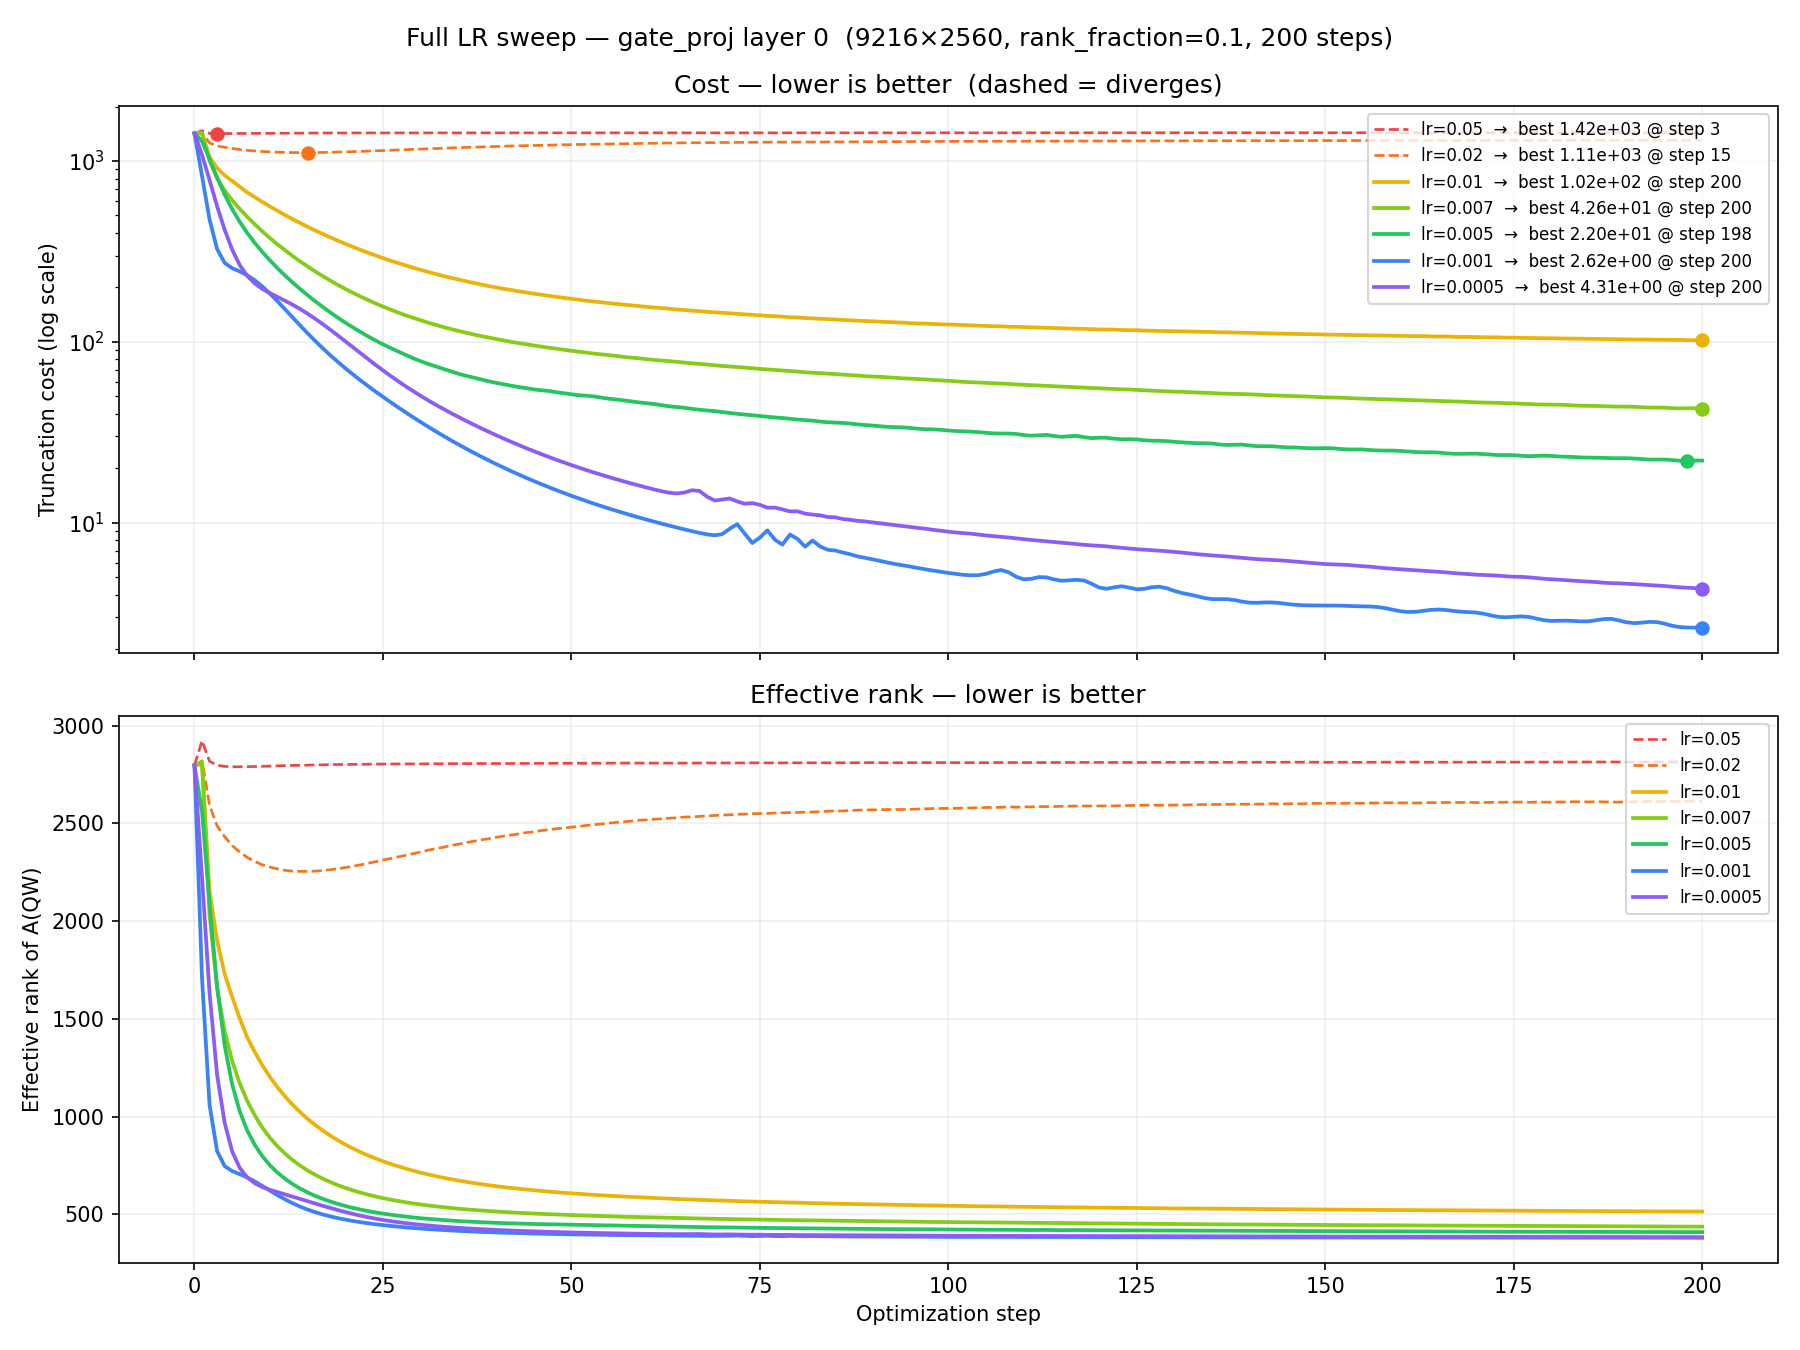
\includegraphics[width=\columnwidth]{lr_sweep.png}
  \caption{Learning-rate sweep for tensor disentanglement (Qwen3.5-0.8B MLP
    layer, 200 steps). Mid-range rates balance convergence speed and
    stability; large rates diverge.}
  \label{fig:lr}
\end{figure}

\textbf{Gauge quality across bake ranks.} The checkpoint's gauge was optimized
at $\rho{=}0.1$ while the interventions bake at $\rho{=}0.25$, so the KL
bound's tightness is not guaranteed at the bake rank
(Section~\ref{sec:wmd}). Measured
on the stored spectra, the advantage transfers: relative to identity-gauge
(plain SVD) truncation in the same bipartition, the optimized gauge reduces
the discarded tail energy to $0.60\times$ ($\rho{=}0.1$) and $0.58\times$
($\rho{=}0.25$) on \texttt{layers.0.down\_proj}, and to $0.026\times$ and
$0.025\times$ on \texttt{layers.31.up\_proj}---large (if heterogeneous across
layers) and essentially rank-independent.

\textbf{MMLU vs.\ rank.} On Qwen3.5-4B (5-shot, 5 questions per subtask),
accuracy stays near the base model's 0.737 down to $\rho \approx 0.5$, then
degrades monotonically to 0.42 at $\rho{=}0.1$---still above the 0.25 random
baseline (Figure~\ref{fig:mmlu}).

\textbf{Coherence cliff.} Free-running generation tells a sharper story than
likelihood-based MMLU: at $\rho{=}0.1$ every inspected generation collapses
into degenerate repetition, while at $\rho \geq 0.25$ generations are fluent,
structured solutions. Consistently, the Novice's teacher-forced flip rate on
Master rollouts falls from 44.0\% at $\rho{=}0.1$ (disagreement smeared over
half the tokens, i.e., noise) to 12.3\% at $\rho{=}0.25$ (concentrated
disagreement). We therefore run all interventions at $\rho{=}0.25$, the
sharpest coherent operating point: the Novice is far weaker than the Master
generatively---released on the Master's own trajectories it completes them
correctly only 26\% of the time (E1 below), versus 100\% for the Master by
construction---yet its disagreements are attributable to specific positions
rather than global incoherence.

\begin{figure}[t]
  \centering
  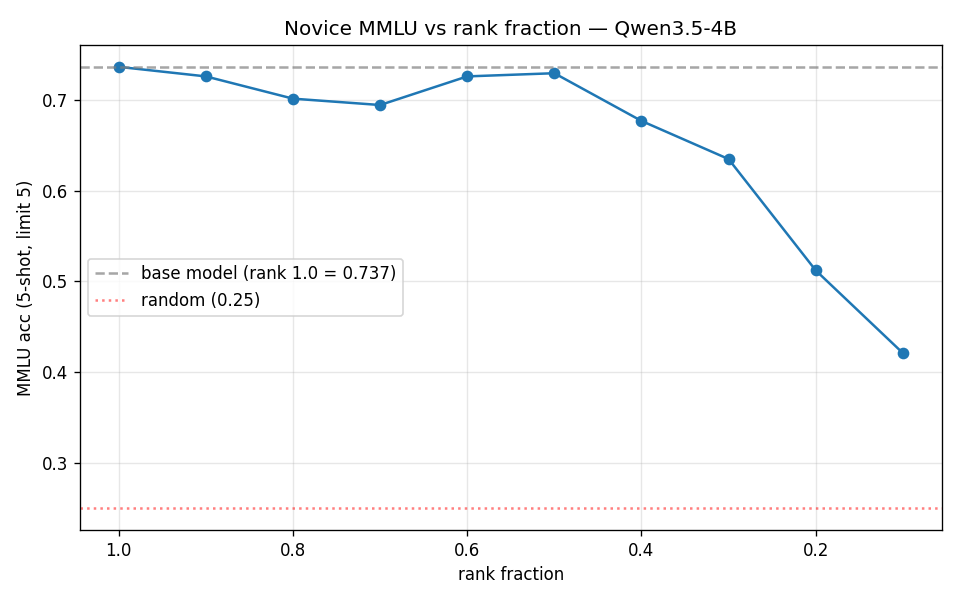
\includegraphics[width=0.85\columnwidth]{mmlu_rank_sweep.png}
  \caption{MMLU accuracy vs.\ Novice rank fraction on Qwen3.5-4B
    (\texttt{lm-eval}, 5-shot, 5 questions per subtask). Accuracy is preserved
    until $\rho \approx 0.5$, then degrades; note that at $\rho{=}0.1$ the
    Novice still scores above chance on likelihood ranking even though its
    free-running generation is degenerate.}
  \label{fig:mmlu}
\end{figure}

\SubSection{Intervention experiments}\label{sec:intervention-results}

Table~\ref{tab:outcome} summarizes the outcome-level results of all three
experiments; Table~\ref{tab:graded} reports E2's graded per-token metrics.

\begin{table}[t]
  \small
  \centering
  \begin{tabular}{llcc}
    \toprule
    Exp. & Arm & Rate & Count \\
    \midrule
    E1 (success$\uparrow$) & release at flip      & 0.261 & 30/115 \\
                           & release at control   & 0.270 & 31/115 \\
    \midrule
    E2 (break$\downarrow$) & flip, Novice token   & 0.241 & 7/29 \\
                           & flip, rank-2 token   & 0.100 & 3/30 \\
                           & control, rank-2      & 0.194 & 6/31 \\
    \midrule
    E3 (break$\downarrow$) & flip-dense step      & 0.151 & 8/53 \\
                           & control step         & 0.176 & 9/51 \\
                           & flip-dense, Novice version & 0.152 & 7/46 \\
    \bottomrule
  \end{tabular}
  \caption{Outcome-level intervention results. E1 reports the Novice's
    completion success rate after taking over at the given position (H1
    predicts \emph{lower} success at flips). E2/E3 report the rate at which the
    Master's free-run no longer reaches the correct answer after the
    perturbation (H1 predicts \emph{higher} break rates at flips). No
    comparison is significant; exact tests in the text.}
  \label{tab:outcome}
\end{table}

\begin{table}[t]
  \small
  \centering
  \begin{tabular}{lccc}
    \toprule
    E2 arm & Local disr. & Answer drop & $H_M$ \\
           & (nats/tok)  & (nats/tok)  &       \\
    \midrule
    flip, Novice token & 2.56 & 0.0009 & 0.41 \\
    flip, rank-2       & 2.55 & 0.0009 & 0.41 \\
    control, rank-2    & 1.60 & 0.0013 & 0.08 \\
    \bottomrule
  \end{tabular}
  \caption{E2 graded metrics (means over 115 trials per arm). Local disruption
    differs between flip and control positions; the answer-tied drop is
    negligible for every arm. $H_M$: mean Master entropy at the perturbed
    position, confirming that flips sit at high-entropy positions---hence the
    entropy-adjusted analyses in the text.}
  \label{tab:graded}
\end{table}

\textbf{E1: no release-point effect.} Success after handing over at a flip was
30/115 (0.261; Wilson 95\%~CI $[0.189, 0.348]$) versus 31/115 (0.270; CI
$[0.197, 0.357]$) at depth-matched controls; paired difference $+0.009$. Of
115 pairs, 108 were concordant; the discordant pairs split 4 (control
succeeded, flip failed) versus 3 (the reverse), McNemar exact test
$p = 1.00$. Success is instead governed by release depth
(Figure~\ref{fig:release}): in the deepest quartile of release positions both
arms succeed at $\approx 0.7$, in the earliest at $\approx 0$--$0.1$. H1 is
not supported at this granularity.

\begin{figure}[t]
  \centering
  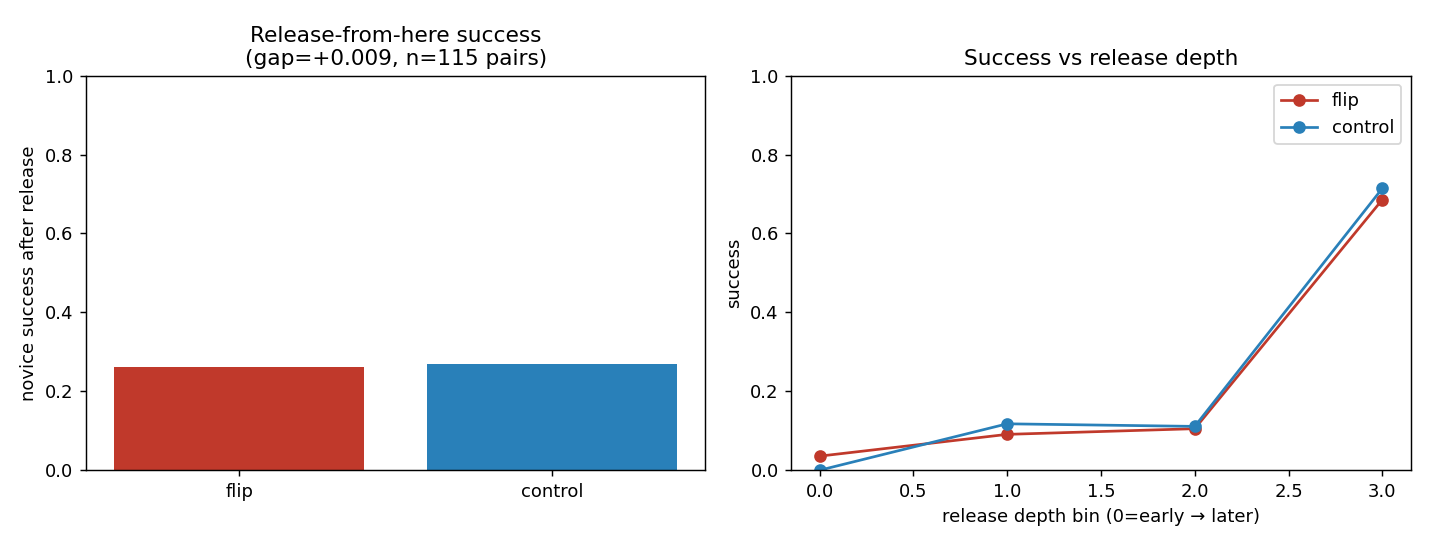
\includegraphics[width=\columnwidth]{e1_release_depth.png}
  \caption{E1 (release-from-here). Left: Novice completion success after
    taking over at flip vs.\ depth-matched control positions (115 pairs)---no
    difference. Right: success by release-depth quartile (bin 0 = earliest
    quarter of the rollout). Both arms rise identically with depth: the
    outcome is governed by how much of the Master's trajectory the Novice
    inherits, not by whether the release point is a flip.}
  \label{fig:release}
\end{figure}

\textbf{E2: a local but not an outcome effect.} Perturbing at a flip disrupts
the Master's immediate continuation substantially more than at a matched
control (2.55 vs.\ 1.60 nats/token, Table~\ref{tab:graded}). Flips sit at
higher-entropy positions ($H_M$ 0.41 vs.\ 0.08), and entropy independently
predicts disruption ($\beta_2 = 0.97$, SE $0.36$, $t = 2.69$), but the flip
effect survives the adjustment: $\beta_1 = 0.62$, SE $0.26$, $t = 2.35$
($n{=}230$), and the flip$>$control ordering holds within every entropy
tercile. The effect does not reach the outcome, however: the answer-tied drop
is $\sim$0.001 nats/token in \emph{every} arm, with no flip effect
($\beta_1 = -0.0002$, SE $0.0017$, $t = -0.14$, $n{=}225$),
and the free-run answer-break subset shows no coherent ordering (7/29, 3/30,
6/31). The Novice's specific token adds nothing over the Master's own second
choice at the same position: the paired difference is $+0.017$ nats/token
locally (Novice larger in only 18\% of pairs) and $+0.0001$ on the answer
metric (11\% of pairs).

\textbf{E3: no step-level effect.} Corrupting a flip-dense reasoning step broke
the final answer in 8/53 free-runs (0.151; CI $[0.079, 0.271]$) versus 9/51
(0.176; CI $[0.096, 0.303]$) for depth-matched low-disagreement steps; Fisher
exact odds ratio 0.83, $p = 0.80$---directionally \emph{opposite} to H1.
Replacing a flip-dense step by the Novice's own version of it was
indistinguishable from generic corruption of the same step (7/46 vs.\ 8/53;
Fisher $p = 1.00$; on the paired answer-drop metric the Novice version was
larger in only 10\% of step pairs). The entropy-adjusted answer-drop OLS is
likewise null ($\beta_1 = -0.0018$, SE $0.0023$, $t = -0.79$, $n{=}137$). Notably, the Master
recovered the correct answer after whole-step corruption in 84\% of all trials
(126/150), independent of the step's flip density.


\Section{Discussion}

\SubSection{What the results mean for H1}

Across three intervention designs of increasing strength---and in particular in
E3, whose free-running outcome metric gives downstream reasoning every chance
to amplify a corrupted step---we consistently fail to reject the null. Where
the Novice disagrees with the Master is, causally, not where the outcome is
decided: flip positions and flip-dense steps are no more outcome-critical than
depth-matched controls, and the Novice's specific alternatives are no more
damaging than the Master's own second choices. We conclude that naive
top-1-flip divergence, used as a per-token or per-step credit weight, would
not concentrate learning where it matters, and an RL run built on it would
most likely reproduce a uniform-weighting baseline at extra cost.

Two genuine findings survive alongside the negative. First, disagreement
positions are \emph{locally} special: perturbations there disrupt the
immediate continuation about 60\% more than at matched positions, beyond what
Master entropy explains. Divergence therefore does measure something real
about where the truncated capacity acts---it just measures local fragility,
not outcome leverage. Second, the Master is strikingly robust on MATH-500:
even corrupting an entire reasoning step leaves the final answer intact
84\% of the time. Only a small minority of steps is load-bearing, and
identifying them evidently requires more than capacity-difference signals.

On the relation to entropy: our data do \emph{not} show that entropy is a
sufficient credit signal either. Entropy predicted local disruption, but
neither entropy nor flips predicted the outcome-tied metrics---on those,
everything was null. The correct summary is that divergence and entropy are
correlated, each carries independent \emph{local} information, and neither, in
our setting, identifies outcome-critical positions. This is consistent with
the interpretation of high-entropy tokens as \emph{forks} whose importance is
realized over many rollouts during training~\cite{wang2025forking}, rather
than as counterfactually decisive positions within a single trajectory.

\SubSection{Why the hypothesis may fail}

The premise behind H1 conflates two notions of importance: a step can be hard
\emph{for a weaker model to produce} without being critical \emph{to the
outcome}. Much of what extra MLP capacity buys appears to be fluency and
confidence at delicate positions---exactly what the local-disruption effect
detects---while the mathematically decisive content is either redundantly
encoded across the trajectory (the Master re-derives it after corruption) or
concentrated in a few steps that flips do not preferentially mark. TIP's
setting~\cite{xu2026tip} explains why the same signal can still be valuable in
distillation: there, ``hard for the weaker model'' \emph{is} the training
target, no causal claim needed. For RL credit assignment, our results show
that the causal claim must be established separately, and here it fails.

\SubSection{Limitations}

Our conclusions are bounded by the setting: one Master (Qwen3.5-4B), one
Novice family (MLP-only disentanglement with the gauge optimized at
$\rho{=}0.1$, evaluated chiefly at $\rho{=}0.25$, where the truncation
bound's tightness is verified empirically on sampled layers rather than
guaranteed), one dataset (MATH-500; 23 Master-correct rollouts), greedy
decoding, and top-1 flips as the divergence instantiation. The binary outcome metrics have
modest power ($\sim$50--115 per arm; the reported CIs are correspondingly
wide), though the consistency of the null across three designs and both graded
and binary metrics argues against a large hidden effect. The MMLU sweep uses a
fixed 5-question-per-subtask budget, adequate for relative comparisons across
$\rho$ but not for absolute benchmark claims. The answer-tied drop metric
teacher-forces intervening reasoning and is thus conservative by design; the
free-run metrics in E1/E3 are the complementary, unconstrained tests. Finally,
continuous divergence measures (e.g., Jensen--Shannon mass aggregated per
trajectory), sampled rather than greedy rollouts, and other Novice
constructions remain untested and are natural follow-ups.

\SubSection{Outlook}

The infrastructure result stands independently of the negative: Master/Novice
pairs can be produced repeatably at 4B scale, with rank fraction as a smooth,
characterized control knob and a documented coherent operating range. Given
H1's failure, we see three defensible directions: (i)~aggregate rather than
pointwise use of divergence (e.g., trajectory-level divergence mass as a
difficulty or novelty signal); (ii)~combining divergence with signals whose
training-time value is established, such as entropy-based token
selection~\cite{wang2025forking}, where divergence's independent local
information may still help; and (iii)~learned dense-reward approaches in the
PRIME family~\cite{cui2025prime}, against which any future training-free
comparator should be benchmarked. Any of these should be preceded by the same
kind of causal validation we applied here.


\Section{Conclusion}

We formalized the Master/Novice framework for densifying verifiable rewards,
built and validated the tensor-disentanglement pipeline that makes it
practical at 4B scale, and subjected its central premise to a ladder of three
causal intervention tests on MATH-500. The premise did not hold: top-1
disagreement between Master and Novice does not mark outcome-critical
positions or steps (McNemar $p{=}1.00$; Fisher $p{=}0.80$), and the Novice's
specific token choices carry no more leverage than generic perturbations. What
disagreement does mark---robustly, and beyond Master entropy---is local
fragility of the immediate continuation. We report this negative result with
exact statistics because it de-scopes an otherwise attractive idea: dense
rewards from a training-free capacity-reduced comparator cannot be assumed to
target the right tokens, and causal validation of any proposed credit signal
should precede RL integration. The released pipeline, the coherence-cliff
characterization, and the three reusable intervention designs are intended to
make exactly that validation cheap for future signals.


\section*{AI-Use Statement}

AI assistants were used for limited drafting and coding assistance during this
project. Boilerplate and auxiliary code (e.g., plotting, evaluation harness
glue) may have been generated with an LLM, and LLM tools were used to assist
with editing and restructuring the manuscript. All content was reviewed,
modified, and verified by the authors, who take full responsibility for the
final work.

\bibliographystyle{main}
\bibliography{main}

\end{document}
